\chapter{Validation}
\label{ch:validation}
Nous désirons mesurer deux aspects de notre programme : la qualité des stratégies décrites dans le sujet de \ac{TP} et la complexité de chaque algorithme. Pour cela, nous avons mis en place un championnat qui oppose différentes configurations, ainsi que des mesures de complexité pour chaque algorithme. Les statistiques sont obtenues sur 100 itérations, sauf pour certaines profondeurs 6 pour des raisons de temps de calcul. Les résultats sont présentés dans les sections suivantes.


\section{Mesure de complexité : Exploration de l'arbre de jeu}
\label{sec:game_tree_exploration}
Nous comparons ici la complexité en temps et en nombre de nœuds explorés. Nous avons mesuré ces deux aspects sur 24 configurations. Elles correspondent à un affrontement entre soit Minimax, soit Alpha-Beta contre un joueur aléatoire avec une profondeur de recherche de 2, 4 et 6, sur différentes stratégies.


\begin{table}[H]
    \centering
    \caption{NegamaxAlphaBeta/Negamax Analyse comparative du temps d'exécution d'une partie à travers les profondeurs et les stratégies en secondes}
    \resizebox{0.85\textwidth}{!}{% Resize table to fit within the text width, keeping aspect ratio
        \begin{tabular}{
            @{}
            >{\raggedright\arraybackslash}p{1cm}
            >{\raggedright\arraybackslash}p{4cm}
            S
            S
            S
            @{}
            }
            \toprule
            \textbf{Depth} & \textbf{Strategy}           & {\textbf{Mean}}             & {\textbf{Std}}             \\
            \midrule
            \multicolumn{4}{c}{\textbf{Depth 2}}                                                                    \\
            \midrule
                           & Positional                  & {74.10\% (0.03 vs 0.04)}    & {198.71\% (0.02 vs 0.01)}  \\
                           & Absolute                    & {86.94\% (0.01 vs 0.02)}    & {208.26\% (0.02 vs 0.01)}  \\
                           & Mobility                    & {54.55\% (0.06 vs 0.12)}    & {83.37\% (0.02 vs 0.03)}   \\
                           & Mixed (thresholds=[30, 55]) & {67.22\% (0.06 vs 0.08)}    & {140.54\% (0.04 vs 0.03)}  \\
            \midrule
            \multicolumn{4}{c}{\textbf{Depth 4}}                                                                    \\
            \midrule
                           & Positional                  & {14.56\% (0.90 vs 6.21)}    & {14.38\% (0.30 vs 2.06)}   \\
                           & Absolute                    & {24.09\% (0.51 vs 2.10)}    & {16.92\% (0.19 vs 1.15)}   \\
                           & Mobility                    & {13.04\% (1.50 vs 11.52)}   & {11.27\% (0.49 vs 4.38)}   \\
                           & Mixed (thresholds=[30, 55]) & {15.93\% (1.17 vs 7.34)}    & {12.67\% (0.40 vs 3.18)}   \\
            \midrule
            \multicolumn{4}{c}{\textbf{Depth 6}}                                                                    \\
            \midrule
                           & Positional                  & {8.45\% (35.20 vs 416.65)}  & {2.60\% (2.82 vs 108.49)}  \\
                           & Absolute                    & {12.23\% (20.14 vs 164.64)} & {18.39\% (13.95 vs 75.87)} \\
                           & Mobility                    & {2.83\% (39.32 vs 1390.49)} & {1.03\% (7.65 vs 745.69)}  \\
                           & Mixed (thresholds=[30, 55]) & {3.17\% (17.34 vs 546.98)}  & {4.36\% (5.04 vs 115.61)}  \\
            \bottomrule
        \end{tabular}
    }
\end{table}

L'unité est la seconde. Nous avons mesuré le temps de calcul pour chaque partie jouée.


\subsection{Nombre de nœuds explorés}
\label{subsec:node_explored}
Nous avons mesuré à chaque coup des joeurs, le nombre de nœuds explorés. Nous pouvons donc comparer chaque algorithme sur un graphe pour chaque profondeur donnée\footnote{Chaque figure est disponible séparément dans les appendices \ref{app:node_explored}.}. Nous avons également calculé le nombre moyen de nœuds explorés pour chaque configuration. Les résultats sont présentés dans les tableaux \ref{tab:node_explored_summary} et \ref{tab:node_explored_summary-2}.

\begin{figure}[H]
    \centering
    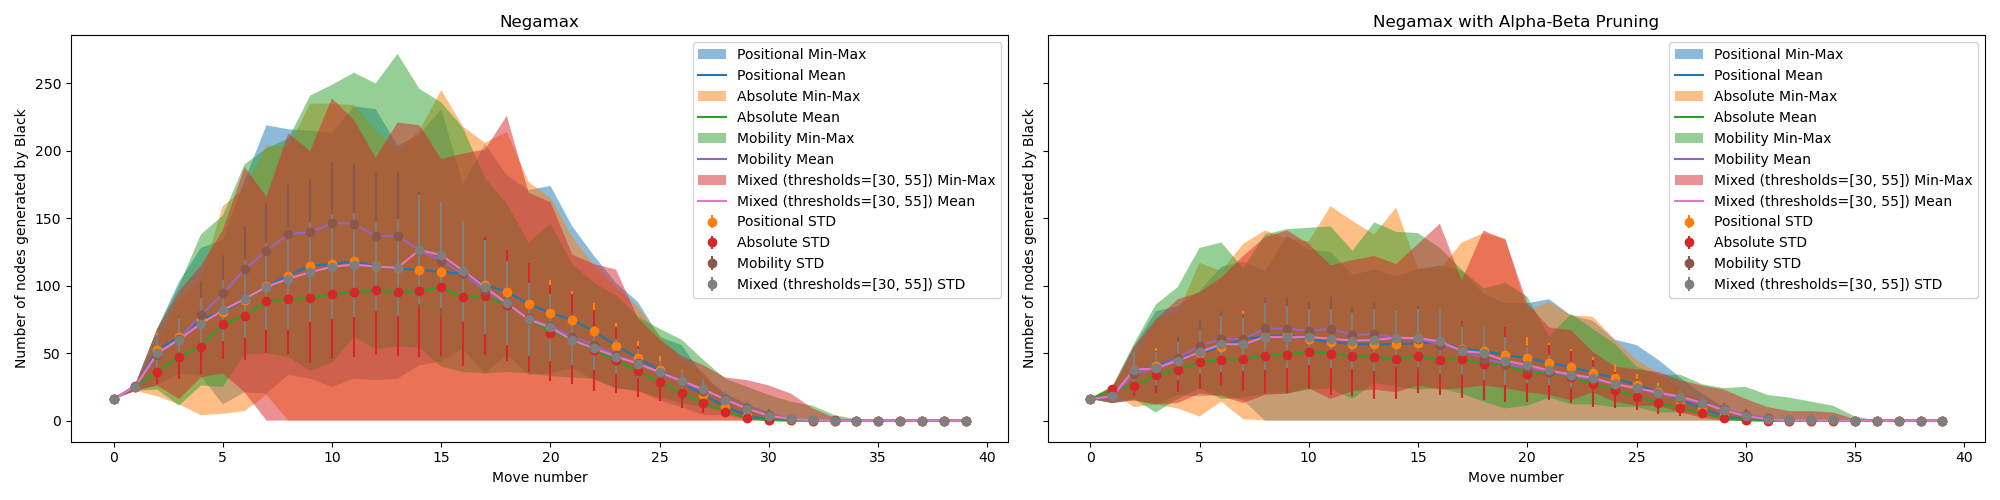
\includegraphics[width=\textwidth]{ressources/Number of nodes generated by Black_depth_2_combined.png}
    \caption{Nombre de nœuds explorés par Minimax et Alpha-Beta en profondeur 2.}
    \label{fig:complexity_node_explored-2}
\end{figure}

\begin{figure}[H]
    \centering
    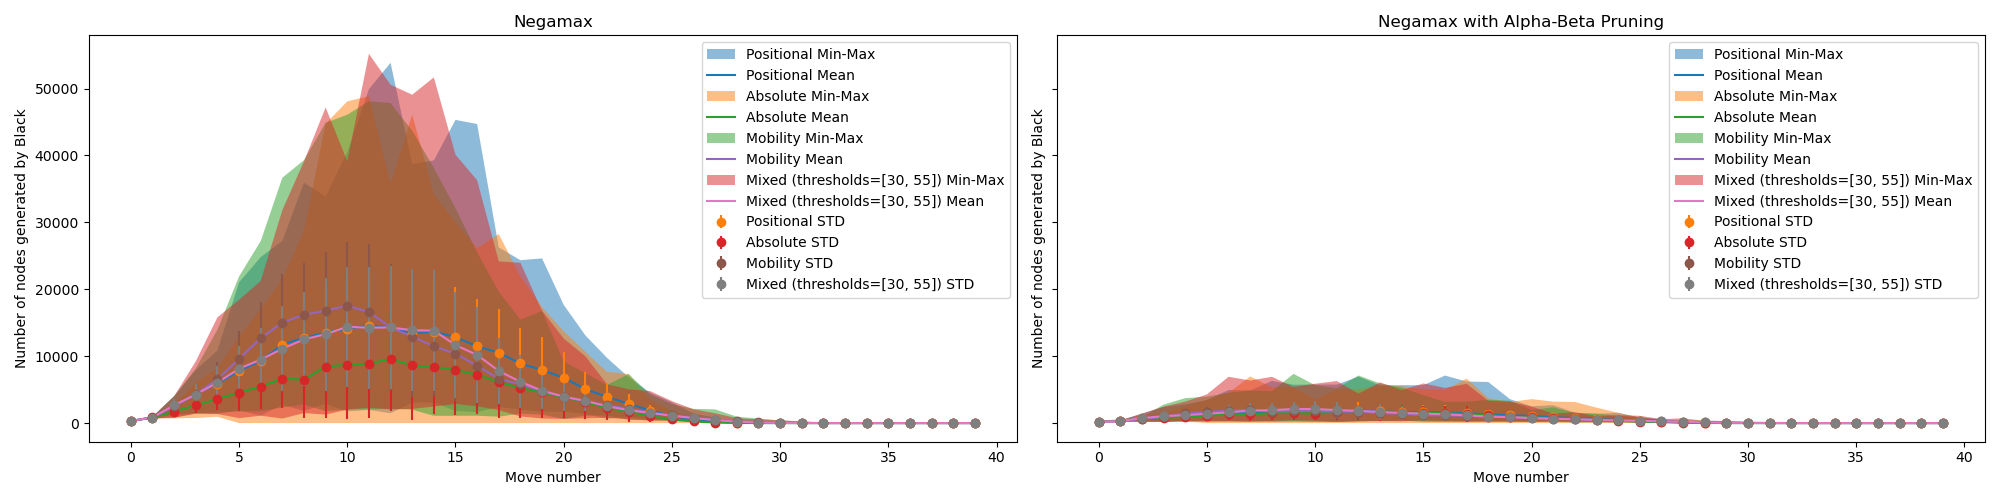
\includegraphics[width=\textwidth]{ressources/Number of nodes generated by Black_depth_4_combined.png}
    \caption{Nombre de nœuds explorés par Minimax et Alpha-Beta en profondeur 4.}
    \label{fig:complexity_node_explored-4}
\end{figure}

\begin{figure}[H]
    \centering
    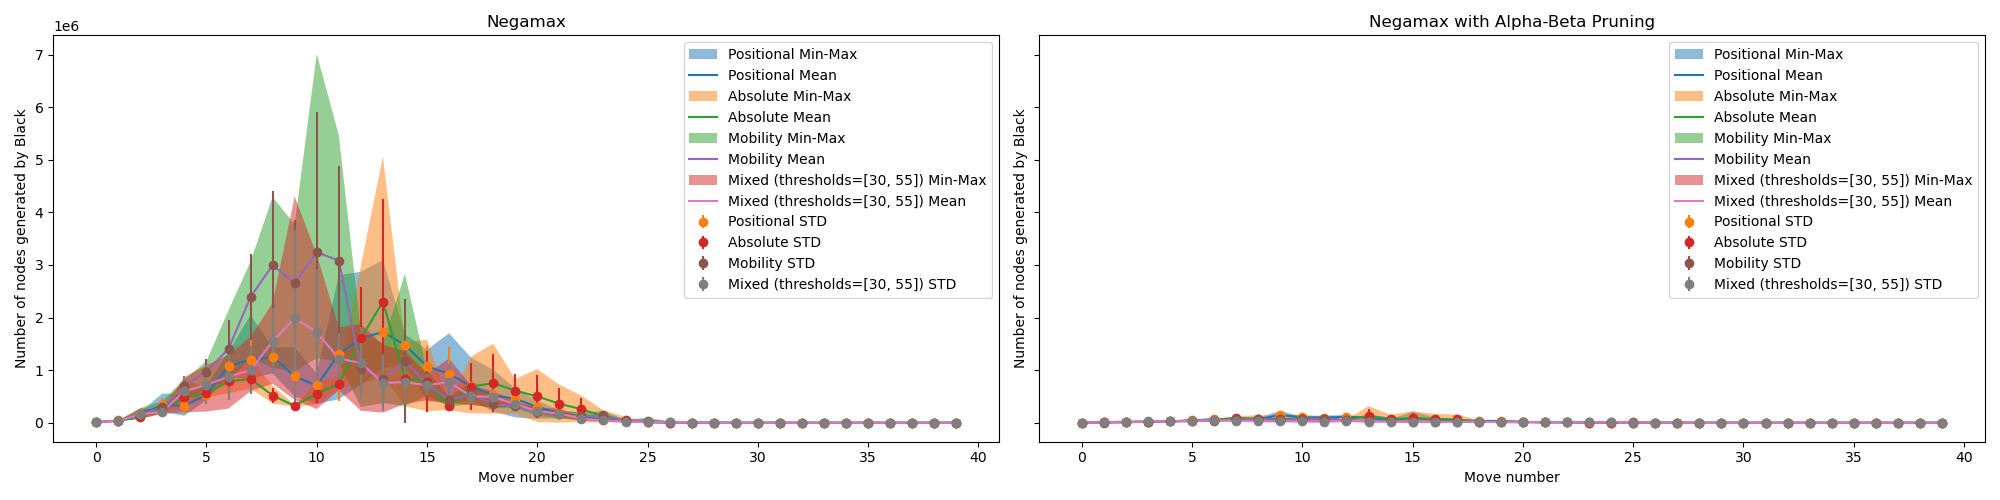
\includegraphics[width=\textwidth]{ressources/Number of nodes generated by Black_depth_6_combined.png}
    \caption{Nombre de nœuds explorés par Minimax et Alpha-Beta en profondeur 6.}
    \label{fig:complexity_node_explored-6}
\end{figure}

Dans un tableau récapitulatif, nous pouvons observer le nombre moyen de nœuds explorés par Minimax et Alpha-Beta pour chaque profondeur. Les résultats sont présentés dans le tableau \ref{tab:node_explored_summary}. Pour les valeurs exactes, voir le tableau \ref{tab:node_explored_summary-2}, avec pour unité $10^4$ le nombre de nœuds explorés.

\begin{table}[H]
    \centering
    \caption{NegamaxAlphaBeta (gauche)/Negamax(droite) Analyse comparative du nombre de nœuds explorés à travers les profondeurs et les stratégies en pourcentage}
    \resizebox{\textwidth}{!}{% Resize table to fit within the text width, keeping aspect ratio
        \begin{tabular}{
            @{}
            >{\raggedright\arraybackslash}p{1cm}
            >{\raggedright\arraybackslash}p{4cm}
            S
            S
            S
            @{}
            }
            \toprule
            \textbf{Depth} & \textbf{Strategy}           & {\textbf{Max of Maxs}} & {\textbf{Mean of Means}} & {\textbf{Mean of Stds}} \\
            \midrule
            \multicolumn{5}{c}{\textbf{Depth 2}}                                                                                       \\
            \cmidrule(lr){1-5}
                           & Positional                  & 58.80\%                & 57.52\%                  & 65.20\%                 \\
                           & Absolute                    & 64.90\%                & 55.79\%                  & 63.92\%                 \\
                           & Mobility                    & 54.04\%                & 53.95\%                  & 60.26\%                 \\
                           & Mixed (thresholds=[30, 55]) & 61.09\%                & 58.35\%                  & 62.72\%                 \\
            \midrule
            \multicolumn{5}{c}{\textbf{Depth 4}}                                                                                       \\
            \cmidrule(lr){1-5}
                           & Positional                  & 13.19\%                & 14.77\%                  & 16.35\%                 \\
                           & Absolute                    & 14.27\%                & 21.19\%                  & 17.92\%                 \\
                           & Mobility                    & 15.29\%                & 14.06\%                  & 14.30\%                 \\
                           & Mixed (thresholds=[30, 55]) & 12.54\%                & 15.76\%                  & 15.56\%                 \\
            \midrule
            \multicolumn{5}{c}{\textbf{Depth 6}}                                                                                       \\
            \cmidrule(lr){1-5}
                           & Positional                  & 7.15\%                 & 6.96\%                   & 6.66\%                  \\
                           & Absolute                    & 6.26\%                 & 7.67\%                   & 10.21\%                 \\
                           & Mobility                    & 1.93\%                 & 2.98\%                   & 2.56\%                  \\
                           & Mixed (thresholds=[30, 55]) & 1.84\%                 & 3.07\%                   & 2.77\%                  \\
            \bottomrule
        \end{tabular}
    }
    \label{tab:node_explored_summary}
\end{table}

\begin{table}[H]
    \centering
    \caption{NegamaxAlphaBeta (gauche)/Negamax(droite) Analyse comparative du nombre de nœuds explorés à travers les profondeurs et les stratégies en valeur exacte}
    \resizebox{\textwidth}{!}{% Resize table to fit within the text width, keeping aspect ratio
        \begin{tabular}{
            @{}
            >{\raggedright\arraybackslash}p{1cm}
            >{\raggedright\arraybackslash}p{4cm}
            S
            S
            S
            @{}
            }
            \toprule
            \textbf{Depth} & \textbf{Strategy}           & {\textbf{Max of Maxs}} & {\textbf{Mean of Means}} & {\textbf{Mean of Stds}} \\
            \midrule
            \multicolumn{5}{c}{\textbf{Depth 2}}                                                                                       \\
            \cmidrule(lr){1-5}
                           & Positional                  & {0.0137 vs 0.0233}     & {0.003193 vs 0.005551}   & {0.001091 vs 0.001673}  \\
                           & Absolute                    & {0.0159 vs 0.0245}     & {0.002579 vs 0.004622}   & {0.001411 vs 0.002208}  \\
                           & Mobility                    & {0.0147 vs 0.0272}     & {0.003256 vs 0.006036}   & {0.001102 vs 0.001830}  \\
                           & Mixed (thresholds=[30, 55]) & {0.0146 vs 0.0239}     & {0.003178 vs 0.005445}   & {0.001087 vs 0.001734}  \\
            \midrule
            \multicolumn{5}{c}{\textbf{Depth 4}}                                                                                       \\
            \cmidrule(lr){1-5}
                           & Positional                  & {0.7103 vs 5.3861}     & {0.078708 vs 0.532977}   & {0.046724 vs 0.285685}  \\
                           & Absolute                    & {0.6975 vs 4.8871}     & {0.068316 vs 0.3224}     & {0.046545 vs 0.259710}  \\
                           & Mobility                    & {0.7352 vs 4.8096}     & {0.073940 vs 0.525755}   & {0.040591 vs 0.283905}  \\
                           & Mixed (thresholds=[30, 55]) & {0.6921 vs 5.5201}     & {0.077103 vs 0.489311}   & {0.044621 vs 0.286737}  \\
            \midrule
            \multicolumn{5}{c}{\textbf{Depth 6}}                                                                                       \\
            \cmidrule(lr){1-5}
                           & Positional                  & {22.08 vs 309.04}      & {2.96 vs 42.50}          & {1.13 vs 16.93}         \\
                           & Absolute                    & {31.68 vs 506.37}      & {2.77 vs 36.06}          & {1.98 vs 19.34}         \\
                           & Mobility                    & {13.56 vs 701.55}      & {1.79 vs 60.19}          & {0.779 vs 30.44}        \\
                           & Mixed (thresholds=[30, 55]) & {7.90 vs 430.26}       & {1.24 vs 40.39}          & {0.582 vs 20.99}        \\
            \bottomrule
        \end{tabular}
    }
    \label{tab:node_explored_summary-2}
\end{table}



\section{Championnat : Comparaison des algorithmes}
\label{sec:championship}

